% SPDX-License-Identifier: LPPL-1.3a

\documentclass[conference, a4paper]{IEEEtran}
% Add the compsoc option for Computer Society conferences.
%
% If IEEEtran.cls has not been installed into the LaTeX system files,
% manually specify the path to it like:
% \documentclass[conference]{../sty/IEEEtran}

\IEEEoverridecommandlockouts
%\usepackage{graphicx}

	% Turkce karakterler icin.
	\usepackage[turkish]{babel}
	\usepackage[utf8]{inputenc} % Kullanılan encodinge göre utf8 yerine latin5 de yazılabilir.
	\usepackage[T1]{fontenc}

\usepackage{listings}
%\usepackage{etoolbox}
%\let\oldincludegraphics\includegraphics
%\renewcommand{\includegraphics}[2][]{%
%	\oldincludegraphics[#1]{#2}%
%	\shorthandon{=}%
%}
%\pretocmd{\includegraphics}{\shorthandoff{=}}{%}{}

%\uccode `\i='235
%\lccode `\I='031
%\addto\extrasturkish{\uccode`i=\string"9D \lccode`I=\string"19 }
%\addto\noextrasturkish{\uccode`i=`I \lccode`I=`i }


% Some very useful LaTeX packages include:
% (uncomment the ones you want to load)


% *** MISC UTILITY PACKAGES ***
%
%\usepackage{ifpdf}
% Heiko Oberdiek's ifpdf.sty is very useful if you need conditional
% compilation based on whether the output is pdf or dvi.
% usage:
% \ifpdf
%   % pdf code
% \else
%   % dvi code
% \fi
% The latest version of ifpdf.sty can be obtained from:
% http://www.ctan.org/tex-archive/macros/latex/contrib/oberdiek/
% Also, note that IEEEtran.cls V1.7 and later provides a builtin
% \ifCLASSINFOpdf conditional that works the same way.
% When switching from latex to pdflatex and vice-versa, the compiler may
% have to be run twice to clear warning/error messages.






% *** CITATION PACKAGES ***
%
\usepackage{cite}

% *** GRAPHICS RELATED PACKAGES ***
%
\ifCLASSINFOpdf
  \usepackage[pdftex]{graphicx}
  % declare the path(s) where your graphic files are
  % \graphicspath{{../pdf/}{../jpeg/}}
  % and their extensions so you won't have to specify these with
  % every instance of \includegraphics
  % \DeclareGraphicsExtensions{.pdf,.jpeg,.png}
\else
  % or other class option (dvipsone, dvipdf, if not using dvips). graphicx
  % will default to the driver specified in the system graphics.cfg if no
  % driver is specified.
  % \usepackage[dvips]{graphicx}
  % declare the path(s) where your graphic files are
  % \graphicspath{{../eps/}}
  % and their extensions so you won't have to specify these with
  % every instance of \includegraphics
  % \DeclareGraphicsExtensions{.eps}
\fi
% graphicx was written by David Carlisle and Sebastian Rahtz. It is
% required if you want graphics, photos, etc. graphicx.sty is already
% installed on most LaTeX systems. The latest version and documentation can
% be obtained at:
% http://www.ctan.org/tex-archive/macros/latex/required/graphics/
% Another good source of documentation is "Using Imported Graphics in
% LaTeX2e" by Keith Reckdahl which can be found as epslatex.ps or
% epslatex.pdf at: http://www.ctan.org/tex-archive/info/
%
% latex, and pdflatex in dvi mode, support graphics in encapsulated
% postscript (.eps) format. pdflatex in pdf mode supports graphics
% in .pdf, .jpeg, .png and .mps (metapost) formats. Users should ensure
% that all non-photo figures use a vector format (.eps, .pdf, .mps) and
% not a bitmapped formats (.jpeg, .png). IEEE frowns on bitmapped formats
% which can result in "jaggedy"/blurry rendering of lines and letters as
% well as large increases in file sizes.
%
% You can find documentation about the pdfTeX application at:
% http://www.tug.org/applications/pdftex





% *** MATH PACKAGES ***
%
\usepackage[cmex10]{amsmath}
% A popular package from the American Mathematical Society that provides
% many useful and powerful commands for dealing with mathematics. If using
% it, be sure to load this package with the cmex10 option to ensure that
% only type 1 fonts will utilized at all point sizes. Without this option,
% it is possible that some math symbols, particularly those within
% footnotes, will be rendered in bitmap form which will result in a
% document that can not be IEEE Xplore compliant!
%
% Also, note that the amsmath package sets \interdisplaylinepenalty to 10000
% thus preventing page breaks from occurring within multiline equations. Use:
%\interdisplaylinepenalty=2500
% after loading amsmath to restore such page breaks as IEEEtran.cls normally
% does. amsmath.sty is already installed on most LaTeX systems. The latest
% version and documentation can be obtained at:
% http://www.ctan.org/tex-archive/macros/latex/required/amslatex/math/





% *** SPECIALIZED LIST PACKAGES ***
%
%\usepackage{algorithmic}
% algorithmic.sty was written by Peter Williams and Rogerio Brito.
% This package provides an algorithmic environment fo describing algorithms.
% You can use the algorithmic environment in-text or within a figure
% environment to provide for a floating algorithm. Do NOT use the algorithm
% floating environment provided by algorithm.sty (by the same authors) or
% algorithm2e.sty (by Christophe Fiorio) as IEEE does not use dedicated
% algorithm float types and packages that provide these will not provide
% correct IEEE style captions. The latest version and documentation of
% algorithmic.sty can be obtained at:
% http://www.ctan.org/tex-archive/macros/latex/contrib/algorithms/
% There is also a support site at:
% http://algorithms.berlios.de/index.html
% Also of interest may be the (relatively newer and more customizable)
% algorithmicx.sty package by Szasz Janos:
% http://www.ctan.org/tex-archive/macros/latex/contrib/algorithmicx/




% *** ALIGNMENT PACKAGES ***
%
%\usepackage{array}
% Frank Mittelbach's and David Carlisle's array.sty patches and improves
% the standard LaTeX2e array and tabular environments to provide better
% appearance and additional user controls. As the default LaTeX2e table
% generation code is lacking to the point of almost being broken with
% respect to the quality of the end results, all users are strongly
% advised to use an enhanced (at the very least that provided by array.sty)
% set of table tools. array.sty is already installed on most systems. The
% latest version and documentation can be obtained at:
% http://www.ctan.org/tex-archive/macros/latex/required/tools/


%\usepackage{mdwmath}
%\usepackage{mdwtab}
% Also highly recommended is Mark Wooding's extremely powerful MDW tools,
% especially mdwmath.sty and mdwtab.sty which are used to format equations
% and tables, respectively. The MDWtools set is already installed on most
% LaTeX systems. The lastest version and documentation is available at:
% http://www.ctan.org/tex-archive/macros/latex/contrib/mdwtools/


% IEEEtran contains the IEEEeqnarray family of commands that can be used to
% generate multiline equations as well as matrices, tables, etc., of high
% quality.


%\usepackage{eqparbox}
% Also of notable interest is Scott Pakin's eqparbox package for creating
% (automatically sized) equal width boxes - aka "natural width parboxes".
% Available at:
% http://www.ctan.org/tex-archive/macros/latex/contrib/eqparbox/





% *** SUBFIGURE PACKAGES ***
%\usepackage[tight,footnotesize]{subfigure}
% subfigure.sty was written by Steven Douglas Cochran. This package makes it
% easy to put subfigures in your figures. e.g., "Figure 1a and 1b". For IEEE
% work, it is a good idea to load it with the tight package option to reduce
% the amount of white space around the subfigures. subfigure.sty is already
% installed on most LaTeX systems. The latest version and documentation can
% be obtained at:
% http://www.ctan.org/tex-archive/obsolete/macros/latex/contrib/subfigure/
% subfigure.sty has been superceeded by subfig.sty.



%\usepackage[caption=false]{caption}
%\usepackage[font=footnotesize]{subfig}
% subfig.sty, also written by Steven Douglas Cochran, is the modern
% replacement for subfigure.sty. However, subfig.sty requires and
% automatically loads Axel Sommerfeldt's caption.sty which will override
% IEEEtran.cls handling of captions and this will result in nonIEEE style
% figure/table captions. To prevent this problem, be sure and preload
% caption.sty with its "caption=false" package option. This is will preserve
% IEEEtran.cls handing of captions. Version 1.3 (2005/06/28) and later
% (recommended due to many improvements over 1.2) of subfig.sty supports
% the caption=false option directly:
%\usepackage[caption=false,font=footnotesize]{subfig}
%
% The latest version and documentation can be obtained at:
% http://www.ctan.org/tex-archive/macros/latex/contrib/subfig/
% The latest version and documentation of caption.sty can be obtained at:
% http://www.ctan.org/tex-archive/macros/latex/contrib/caption/




% *** FLOAT PACKAGES ***
%
%\usepackage{fixltx2e}
% fixltx2e, the successor to the earlier fix2col.sty, was written by
% Frank Mittelbach and David Carlisle. This package corrects a few problems
% in the LaTeX2e kernel, the most notable of which is that in current
% LaTeX2e releases, the ordering of single and double column floats is not
% guaranteed to be preserved. Thus, an unpatched LaTeX2e can allow a
% single column figure to be placed prior to an earlier double column
% figure. The latest version and documentation can be found at:
% http://www.ctan.org/tex-archive/macros/latex/base/



%\usepackage{stfloats}
% stfloats.sty was written by Sigitas Tolusis. This package gives LaTeX2e
% the ability to do double column floats at the bottom of the page as well
% as the top. (e.g., "\begin{figure*}[!b]" is not normally possible in
% LaTeX2e). It also provides a command:
%\fnbelowfloat
% to enable the placement of footnotes below bottom floats (the standard
% LaTeX2e kernel puts them above bottom floats). This is an invasive package
% which rewrites many portions of the LaTeX2e float routines. It may not work
% with other packages that modify the LaTeX2e float routines. The latest
% version and documentation can be obtained at:
% http://www.ctan.org/tex-archive/macros/latex/contrib/sttools/
% Documentation is contained in the stfloats.sty comments as well as in the
% presfull.pdf file. Do not use the stfloats baselinefloat ability as IEEE
% does not allow \baselineskip to stretch. Authors submitting work to the
% IEEE should note that IEEE rarely uses double column equations and
% that authors should try to avoid such use. Do not be tempted to use the
% cuted.sty or midfloat.sty packages (also by Sigitas Tolusis) as IEEE does
% not format its papers in such ways.





% *** PDF, URL AND HYPERLINK PACKAGES ***
%
%\usepackage{url}
% url.sty was written by Donald Arseneau. It provides better support for
% handling and breaking URLs. url.sty is already installed on most LaTeX
% systems. The latest version can be obtained at:
% http://www.ctan.org/tex-archive/macros/latex/contrib/misc/
% Read the url.sty source comments for usage information. Basically,
% \url{my_url_here}.

% *** Do not adjust lengths that control margins, column widths, etc. ***
% *** Do not use packages that alter fonts (such as pslatex).         ***
% There should be no need to do such things with IEEEtran.cls V1.6 and later.
% (Unless specifically asked to do so by the journal or conference you plan
% to submit to, of course. )
\usepackage{multirow}
\usepackage{array}
\usepackage[lofdepth,lotdepth]{subfig}

% correct bad hyphenation here
\hyphenation{op-tical net-works semi-conduc-tor}

\setlength{\textfloatsep}{5pt}

%\renewcommand{\tablename}{TABLO}
\AtBeginDocument{%
  \renewcommand\tablename{TABLO}
}

\AtBeginDocument{%
  \renewcommand\abstractname{Abstract}
}

\begin{document}

%\IEEEpubid{\makebox[\columnwidth]{978-1-5090-1679-2/16/\$31.00 ©2016 IEEE\hfill}
%\hspace{\columnsep}\makebox[\columnwidth]{}}

%
% paper title
% can use linebreaks \\ within to get better formatting as desired
\title{Çevreci Gömülü Sistemler için Enerji Optimizasyonu: Algoritmaların Zaman Karmaşılıklığı ile Enerji Tüketimleri Arasındaki İlişkinin İncelenmesi\\
Energy Optimization for Green Embedded Systems: Investigation of the Relationship Between Time Complexity and Power Usage}

% author names and affiliations
% use a multiple column layout for up to three different
% affiliations
\author{\IEEEauthorblockN{\textit{Yazarlar Gizlenmiştir}}
\IEEEauthorblockA{\\
\\
\\
\\
\\
}
}

% conference papers do not typically use \thanks and this command
% is locked out in conference mode. If really needed, such as for
% the acknowledgment of grants, issue a \IEEEoverridecommandlockouts
% after \documentclass

% for over three affiliations, or if they all won't fit within the width
% of the page, use this alternative format:
%
% use for special paper notices
%\IEEEspecialpapernotice{(Invited Paper)}

% make the title area
\maketitle
\begin{ozet}
Güç tüketimi, gömülü/IoT cihazlar için büyük önem arz etmektedir. Geçmişten günümüze bu cihazlar için algoritmalar tercih edilirken teorik zaman karmaşıklığı baz alınmıştır. Peki bu ne kadar isabetlidir? Bu araştırmada Arduino Uno R3 ve R4 mikrodenetleyicileri üzerinde Bubble, Insertion, Merge, Quick, Heap, Gnome, Radix, Shell, Comb ve Pancake Sort algoritmaları çalıştırılmış ve Nordic Power Profiler Kit II kullanılarak anlık çekilen akım ölçülmüştür. Çekilen akım ile verilen gerilim kullanılarak güç tüketimleri hesaplanmıştır. Güç tüketimleri ile zaman karmaşıklıkları arasında korelasyon analizi yapılmış ve [0.98, 1.0] arasında sonuçlar bulunmuştur (p < 0.0001). Bu bulgular sonucunda zaman kullanımı için optimize etmenin güç tüketimini de optimize ettiği kanıtlanmıştır. Farklı büyük dil modellerinin yazdığı kodların da güç tüketim analizleri yapılmış ve bazı öncül sonuçlar elde edilmiştir.
%\boldmath
\end{ozet}
\begin{IEEEanahtar}
gömülü sistemler,
mikrodenetleyici mimarisi,
algoritmalar, verimlilik,
nesnelerin interneti, IoT,
güç tüketimi,
sıralama algoritmaları,
çevreci hesaplama
\end{IEEEanahtar}

\begin{abstract}
Power usage is a crucial point for embedded/IoT devices. Historically, theoretical time complexities were utilized during the choice of algorithm for these devices. But how accurate is this? In this research; Bubble, Insertion, Merge, Quick, Heap, Gnome, Radix, Shell, Comb and Pancake Sort algorithms have been ran on Arduino Uno R3 and R4 and current draws have been measured. Combining this with voltage, total power consumption has been calculated. The results show a [0.98, 1.0] correlation between the theoretical time complexities and power consumptions (p < 0.0001). The results indicate that optimizing for time spent also optimizes for power consumption. Comparison of power consumption of code generated by different large language models have also been analyzed and some preliminary results have been found.
%\boldmath
\end{abstract}
\begin{IEEEkeywords}
embedded systems,
microcontroller architecture,
algorithms, efficiency,
IoT,
power consumption,
sorting algorithms,
green computing
\end{IEEEkeywords}

% IEEEtran.cls defaults to using nonbold math in the Abstract.
% This preserves the distinction between vectors and scalars. However,
% if the conference you are submitting to favors bold math in the abstract,
% then you can use LaTeX's standard command \boldmath at the very start
% of the abstract to achieve this. Many IEEE journals/conferences frown on
% math in the abstract anyway.

% no keywords

% For peer review papers, you can put extra information on the cover
% page as needed:
% \ifCLASSOPTIONpeerreview
% \begin{center} \bfseries EDICS Category: 3-BBND \end{center}
% \fi
%
% For peerreview papers, this IEEEtran command inserts a page break and
% creates the second title. It will be ignored for other modes.
\IEEEpeerreviewmaketitle

\IEEEpubidadjcol


\section{G{\footnotesize İ}r{\footnotesize İ}ş}

Gömülü ve Nesnelerin İnterneti (IoT) cihazlarının günümüz toplumundaki rolü tartışmasız derecede büyüktür. Çamaşır makinelerinden insansız hava araçlarına kadar, bu cihazlar 21. yüzyılın yıldızları haline gelmiştir. 2025 itibarıyla 18,8 milyar cihaz bulunmakta olup, bu sayının 2030 yılına kadar 40 milyara ulaşması öngörülmektedir \cite{iot-market-2024-summer}. Bu tür cihazlar genellikle ya batarya ile çalışmakta ya da güneş enerjisi gibi kısıtlı bir güç kaynağına bağımlı olmaktadır. Dolayısıyla, bu tür cihazların tasarımında en önemli hususlardan biri enerji tüketiminin yönetilmesidir. Başarılı bir gömülü ürün geliştirmek, sistem performansını en üst düzeye çıkarırken enerji kullanımını en aza indirmeyi gerektirir \cite{bces-embedded-performance-energy-consumption-eval}.

Genellikle programların verimliliği, teorik zaman karmaşıklığına ve bellek kısıtlı ortamlarda kullanılan algoritmaların alan karmaşıklığına dayanarak değerlendirilir. Bu alandaki geçmiş araştırmalar çoğunlukla buyruk (instruction) düzeyinde analizlere ve simülasyon tabanlı modellere odaklanmıştır. Bu modeller, eski ve daha kısıtlı mikroişlemciler üzerinde tatmin edici doğruluk seviyelerine ulaşabilse de, modern mimariler için geliştirilmeye açık olduğunu düşünüyoruz. Çünkü modern mimarilerde kodun çalıştırılması; buyruk boru hattı, dallanma tahmini ve önbellek gibi birçok değişkene bağlıdır. Bu nedenle, bu çalışmada daha kanıta dayalı bir yaklaşım benimsenerek modern yazılımların yapı taşlarını oluşturan kapsamlı bir altyordam seti değerlendirilmeye karar verildi. Elde ettiğimiz bulgularla, gömülü yazılım geliştirme sürecinde en uygun algoritmaların seçimine rehberlik edebilecek, ölçüme dayalı bir bilgi deposu oluşturmayı amaçladık. Çalışmamızda sunulan farklı altyordamların gerçek hayattaki enerji tüketimine dair içgörülerin, daha çevreci bir gelecek ve daha yüksek işlem kapasitesine sahip cihazlar için öncü olacağına inanıyoruz.

\section{İlg{\footnotesize İ}l{\footnotesize İ} Çalışmalar}

Gömülü sistemlerde enerji verimliliği, batarya ile çalışan cihazların yaygınlaşması ve çevresel kaygılar nedeniyle onlarca yıldır aktif bir araştırma alanı olmuştur. Tiwari vd. \cite{tiwari-power-analysis}, buyruk düzeyinde enerji tüketimi modellemesi üzerine öncü çalışmalar yaparak, gömülü yazılımların enerji tüketimini öngörmek için temel ve buyruklar arası maliyet konseptlerini geliştirmiştir. Buyruk düzeyindeki bu enerji modeli, yazılım geliştirme sürecinin erken aşamalarında güç optimizasyonuna olanak tanımıştır. Bu temelin üzerine inşa edilen çalışmalar arasında, Steinke vd.'nin \cite{steinke-instruction-level-energy-model} bellek hiyerarşisi etkilerini de içeren modeli yer almaktadır. Bellek erişim desenlerinin toplam enerji tüketimi üzerindeki belirgin etkisini gösteren bu çalışma, buyruk düzeyindeki modellemeye önemli bir katkı sağlamıştır.

Bunse vd.\cite{bunse-no-corr}, sıralama algoritmalarının enerji tüketimini incelediği deneylerde, algoritmanın zaman karmaşıklığı ile enerji tüketimi arasında doğrudan bir korelasyon olmadığını öne sürmüştür. Ancak, bizim araştırmamızda elde edilen bulgular, zaman karmaşıklığının enerji tüketimiyle güçlü bir korelasyon gösterdiğini ve zaman karmaşıklığı optimizasyonunun her iki faktörü de iyileştirdiğini ortaya koymaktadır. Benzer şekilde, Hashimi vd.\cite{hashimi-binary}\cite{hashimi-mergesort} süperbilgisayarlarda enerji verimliliği için algoritmalar üzerinde deneysel bir enerji tüketimi ölçümü gerçekleştirmiştir.

Bu çalışmada, önceki araştırmalar genişletilerek farklı mikroişlemci mimarileri arasında standardize edilmiş kıyaslamalar sunulmaktadır. Ayrıca, gömülü sistemler için büyük dil modelleri (LLM) tarafından üretilen kodların enerji verimliliği değerlendirilmekte ve algoritma optimizasyonu bağlamında daha önce kapsamlı olarak incelenmemiş yenilikçi bir yaklaşım öne sürülmektedir.

\section{Yöntem}

\subsection{Test Cihazları}

\begin{table}[ph]
  \centering
  \caption{\textsc{Test C{\footnotesize İ}hazları ve Özell{\footnotesize İ}kler{\footnotesize İ}}}
  \label{tab:test-cihazlar}
  \begin{tabular}{|c|c|c|c|}
    \hline
    {Cihaz} & {Mikrodenetleyici} & {Mikroişlemci Mimarisi} & {Saat Hızı} \\
    \hline
    R3 & ATmega328P & Atmel AVR (8-bit) & 16MHz \\
    \hline
    R4 & Renesas RA4M1 & ARM®v7E-M (32-bit) & 48MHz'e kadar \\
    \hline
  \end{tabular}
\end{table}

Gömülü sistemlerde enerji tüketimini ve mikrodenetleyici mimarisini incelemek için iki Arduino platformu kullanıldı. İlk cihaz olan Arduino UNO R3 SMD, makale boyunca R3 olarak adlandırılacaktır, 16 MHz frekansında çalışan 8 bitlik ATmega328P mikrodenetleyicisini barındırmaktadır. Program depolama için 32 KB flaş belleğe, çalışma zamanı verileri için 2 KB SRAM'e ve kalıcı veri depolama için 1 KB EEPROM'a sahiptir. R3, çeşitli açılardan sınırlı olmasına rağmen, karmaşık hesaplama gerektirmeyen senaryolarda uygun maliyetli bir alternatif olarak kullanılabilir. Ayrıca; boşta (idle), bekleme (standby) ve güç kapatma gibi düşük güç modlarını destekleyerek, boşta kaldığı süre boyunca enerji tüketimini azaltma imkanı sunmaktadır \cite{atmega328p-datasheet}.

İkinci cihaz olan Arduino UNO R4 Minima, makale boyunca R4 olarak adlandırılacaktır, 32 bit ARM\textsuperscript \textregistered v7E-M mimarisine dayalı Renesas RA4M1 mikrodenetleyicisini kullanmaktadır. 48 MHz frekansında çalışabilen RA4M1, daha yüksek işlem gücü ve geliştirilmiş enerji verimliliği sunmaktadır. Program kodu için 256 KB flaş bellek, çalışma zamanı verileri için 32 KB SRAM ve kalıcı veri depolama için 8 KB EEPROM içermektedir. Bu iki platformun karşılaştırılmasıyla, bellek boyutunun ve mikrodenetleyici mimarisinin enerji tüketimi üzerindeki etkisi analiz edilebilir. R4, daha güçlü donanımıyla enerji tüketimi açısından daha verimlidir ve veri-yoğun işlemler için daha fazla yetenek sunmaktadır \cite{ra4m1-datasheet}.

\subsection{Kıyaslamalar}

\subsubsection{Sıralama Algoritmaları}

Sıralama algoritmaları, özellikle verimlilik ve kaynak kısıtlamalarının büyük önem taşıdığı gömülü sistemlerde, çok çeşitli uygulamalarda kritik bir rol oynar. Gömülü sistemlerde sınırlı olan işlem gücü ve bellek kapasitesi nedeniyle, en uygun sıralama algoritmasının seçilmesi genel performans üzerinde önemli bir etkiye sahiptir. Bu kıyaslamada, 10 popüler sıralama algoritması her iki cihazda da test edildi: Bubble Sort, Insertion Sort, Merge Sort, Quick Sort, Heap Sort, Gnome Sort, Radix Sort, Shell Sort, Comb Sort ve Pancake Sort.

\subsubsection{Kriptografik Algoritmalar}

Gömülü sistemlerde hassas verilerin korunması büyük önem taşıdığı için, kriptografik algoritmalar veri güvenliğini sağlamak açısından kritik bir rol oynar. Bu kıyaslamada, farklı ChaCha şifreleme ve şifre çözme turları (8, 12 ve 20 tur), farklı anahtar uzunluklarında AES şifreleme ve şifre çözümü (128, 192 ve 256 bit) test edilerek çeşitli kriptografik algoritmaların performansı değerlendirildi. Ayrıca AES (128/192/256)-GCM, ChaCha20-Poly1305 ve Acorn128 ile Ascon128 AEAD (ilişkili veri ile kimlik doğrulamalı şifreleme) şemaları da incelendi.

\subsubsection{Büyük Dil Modelleri Tarafından Üretilen Sıralama Algoritmaları}

Geleneksel sıralama algoritmalarını değerlendirmeye ek olarak, büyük dil modellerinin sıralama kodu üretme potansiyelleri de araştırıldı. Üç yaygın olarak bilinen büyük dil modeli; ChatGPT 4o, Gemini 1.5 Flash ve Claude 3.5 Haiku; kullanılarak daha önce değerlendirdiğimiz 10 sıralama algoritması için kod üretmeleri sağlandı. Bu yaklaşımla, gömülü sistemlerde LLM'lerin optimize sıralama algoritması implementasyonu üretme yetkinliğini değerlendirmek ve onları adil bir kıyaslamaya t$\hat{\text{a}}$bi tutmak amaçlandı.

\subsubsection{Diğer Algoritmalar}

Yaygın kullanılan bazı algoritmalar diğer algoritmalar başlığı altında toplandı. LCG (Doğrusal Artıklık Üreteci) ve MT19937 (Mersenne Twister) rastgele sayı üreteçleri, doğrusal ve ikili arama, matris çarpımı, ikili GCD (En Büyük Ortak Bölen), Dijkstra, Karatsuba çarpımı, fibonacci ve faktöriyel algoritmalarının yinelemeli (iterative) ve özyinelemeli (recursive) versiyonları ve temel bir toplama işlemi, programlarda yaygın olarak kullanılan algoritmaların çeşitliliğini temsil edecek şekilde seçildi.

\subsection{Deney ve Ölçüm Düzeni}

Tüm deneylerde, Arduino kartlarından çekilen akımı gerçek zamanlı olarak ölçmek için Nordic® Power Profiler Kit II (makale boyunca PPK olarak anılacaktır) kullanılmıştır. PPK, 100.000 ölçüm/saniye örnekleme hızına, ±200nA hassasiyete ve 1A'e kadar akım ölçme kapasitesine sahiptir \cite{nordic-ppk-datasheet}. Deneylerde PPK kaynak ölçer (sourcemeter) modunda kullanılmış ve Arduino kartlarını 5V’a kadar besleyebilmesi nedeniyle güç kaynağı olarak görev yapmıştır.

\pagebreak

\begin{figure}[h]
	\centering
	\shorthandoff{=}  %\usepackage[turkish]{babel} kullanıldığı için komuta gerek var
	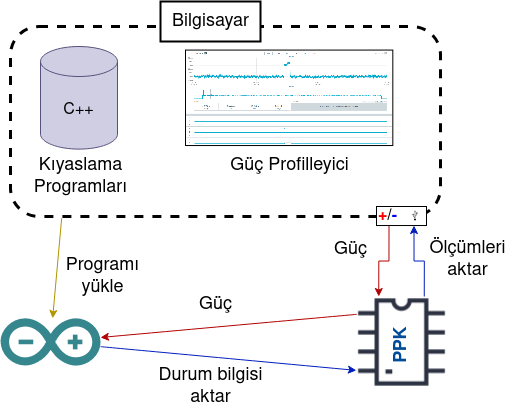
\includegraphics[scale=0.40]{setup-diagram.png}
	\shorthandon{=} %\usepackage[turkish]{babel} kullanıldığı için komuta gerek var
	\caption{Deney düzeneği diyagramı}
	\label{deney-diyagram}
\end{figure}

\figurename~\ref{deney-diyagram}'de gösterildiği gibi, deneyler PPK'yi Arduino kartlarına bağlayarak gerçekleştirildi ve bütün devrenin güç kaynağı olarak bilgisayar kullanıldı. PPK'nin uyarlanabilir kaynak modu sayesinde ise test cihazları deney türüne göre 3,3V ya da 5V pini üzerinden beslenildi. \figurename~\ref{setup-pseudo}'de gösterilen yöntemle ölçümler gerçekleştirildi.


\begin{figure}[h]
	\centering
	\shorthandoff{=}  %\usepackage[turkish]{babel} kullanıldığı için komuta gerek var
	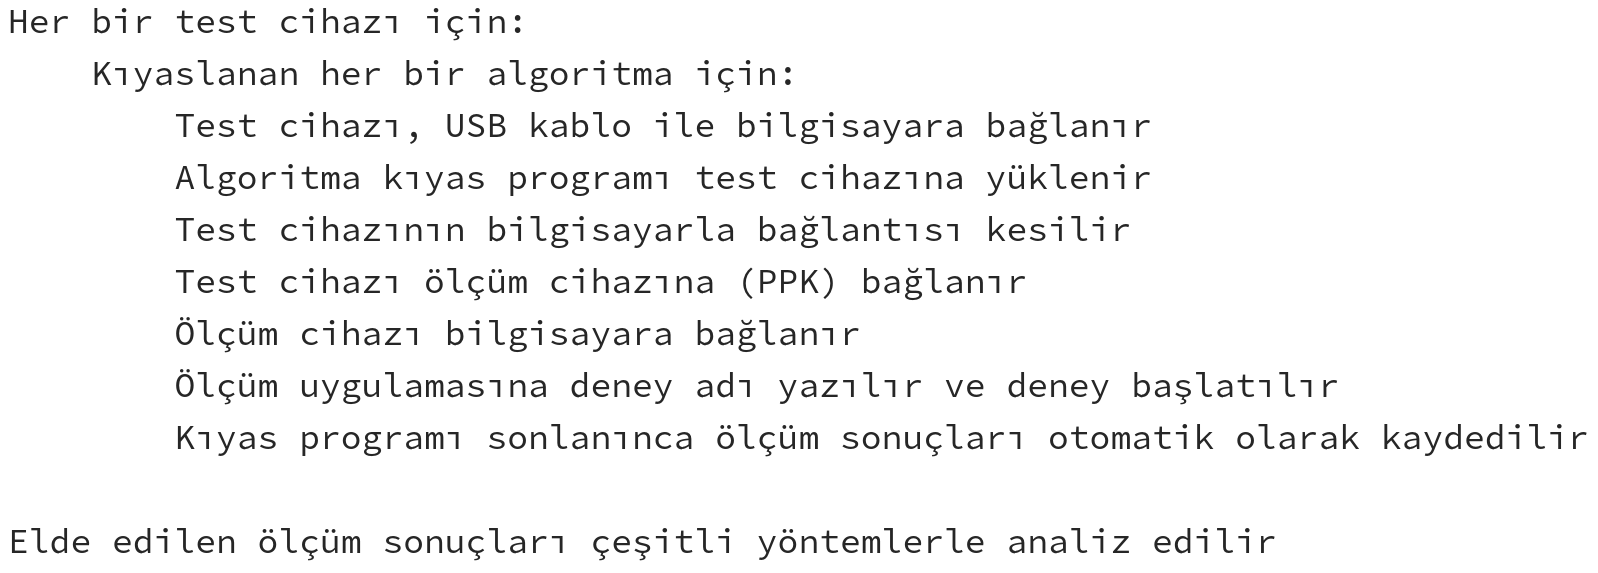
\includegraphics[scale=0.15]{setup-pseudo.png}
	\shorthandon{=} %\usepackage[turkish]{babel} kullanıldığı için komuta gerek var
	\caption{Deney ve ölçüm yöntemi algoritması}
	\label{setup-pseudo}
\end{figure}


\section{Deney Bulguları}

\tablename~\ref{tab:sıralama-algo} incelendiğinde, sıralama algoritmalarına arasında Quick Sort algoritmasının hem en hızlı hem de enerji verimliliği en yüksek algoritma olduğunu görülmüştür. \tablename~\ref{tab:time-complexity-vs-measurements-correlation}’e bakıldığında, algoritmaların teorik zaman karmaşıklığı ile yüksek korelasyonda olduğunu görülmektedir. \tablename~\ref{tab:time-complexity-vs-measurements-correlation-significance}’teki istatiksel anlamlılık verilerine baktığımızda da P değerinin ilgili algoritmaya ait teorik zaman karmaşıklığında en düşük olduğu görülebilmektedir. Sonuçlara bakıldığında, Radix Sort'un zaman karmaşıklığı Quick Sort'tan daha iyi olsa da, {$O(n)$} - {$O(n \log n)$}, Radix Sort'un sabit katsayısının büyüklüğünden dolayı gömülü cihazlarda işlenebilecek veri miktarları için pratikte önemli olmadığını görülmüştür. 

\begin{table}[h]
  \centering
  \caption{\textsc{Sıralama Algor{\footnotesize İ}tmalarının R3 ve R4 Üzer{\footnotesize İ}nde Karşılaştırılması}}
  \label{tab:sıralama-algo}
  \begin{tabular}{|c|c|c|c|c|c|c|}
    \hline
    \multirow{2}{*}{Algoritma$^{\dagger}$} & \multicolumn{2}{c|}{Süre (ms)} & \multicolumn{2}{c|}{Ortalama Güç (mW)} & \multicolumn{2}{c|}{Toplam Enerji ($\mu$J)} \\
    \cline{2-7}
    & R3 & R4 & R3 & R4 & R3 & R4 \\
    \hline
    Quick Sort & 2,32 & 0,30 & 119,006 & 177,647 & 276 & 54 \\
    \hline
    Shell Sort & 3,20 & 0,48 & 119,404 & 171,806 & 382 & 83 \\
    \hline
    Comb Sort & 3,71 & 0,47 & 119,408 & 172,915 & 443 & 81 \\
    \hline
    Heap Sort & 4,68 & 0,56 & 119,850 & 178,518 & 561 & 100 \\
    \hline
    Merge Sort & 5,24 & 0,72 & 118,315 & 172,915 & 620 & 124 \\
    \hline
    Insertion Sort & 5,44 & 0,85 & 119,675 & 178,468 & 651 & 151 \\
    \hline
    Gnome Sort & 18,70 & 2,53 & 120,190 & 173,785 & 2247 & 440 \\
    \hline
    Bubble Sort & 20,80 & 1,89 & 118,656 & 179,626 & 2468 & 339 \\
    \hline
    Pancake Sort & 23,30 & 3,25 & 119,660 & 178,208 & 2788 & 579 \\
    \hline
    Radix Sort & 24,48 & 1,02 & 116,701 & 160,922 & 2857 & 164 \\
    \hline
  \end{tabular}
  \vspace{1mm}

  \raggedright\footnotesize{$^{\dagger}$ R3'te 16 bit, R4'te ise 32 bit büyüklüğe sahip olan 'int' türünde, 128 elemanlı, önceden oluşturulmuş rastgele tam sayı dizisi üzerinde test edilmiştir.}
\end{table}



\begin{table}[h]
  \centering
  \caption{\textsc{Sıralama Algor{\footnotesize İ}tmalarının R4'tek{\footnotesize İ} Performansının Zaman Karmaşıklıkları {\footnotesize İ}le Korelasyonu}}
  \label{tab:time-complexity-vs-measurements-correlation}
  \begin{tabular}{|c|c|c|c|c|}
    \hline
    {Algoritma$^{\dagger}$} & {$O(\log n)$} & {$O(n)$} & {$O(n \log n)$} & {$O(n^2)$} \\
    \hline
    Quick Sort & 0,85 & 1,00 & 1,00 & 0,98 \\
    \hline
    Shell Sort & 0,82 & 0,99 & 1,00 & 0,99 \\
    \hline
    Comb Sort & 0,84 & 1,00 & 1,00 & 0,98 \\
    \hline
    Heap Sort & 0,86 & 1,00 & 1,00 & 0,98 \\
    \hline
    Merge Sort & 0,86 & 1,00 & 1,00 & 0,98 \\
    \hline
    Insertion Sort & 0,74 & 0,97 & 0,98 & 1,00 \\
    \hline
    Gnome Sort & 0,74 & 0,97 & 0,98 & 1,00 \\
    \hline
    Bubble Sort & 0,75 & 0,97 & 0,98 & 1,00 \\
    \hline
    Pancake Sort & 0,75 & 0,97 & 0,98 & 1,00 \\
    \hline
    Radix Sort & 0,88 & 1,00 & 1,00 & 0,97 \\
    \hline
  \end{tabular}
  \vspace{1mm}

  \raggedright\footnotesize{$^{\dagger}$ 8, 16, 32, 64, 128, 256, 512 ve 1024 elemanlı tam sayı listeleri üzerinde koşulmuştur.}
\end{table}


\begin{table}[h]
  \centering
  \caption{\textsc{Sıralama Algor{\footnotesize İ}tmalarının R4'tek{\footnotesize İ} Performansının Zaman Karmaşıklıkları {\footnotesize İ}le Korelasyonlarının {\footnotesize İ}stast{\footnotesize İ}ksel Anlamlılığı}}
  \label{tab:time-complexity-vs-measurements-correlation-significance}
  \begin{tabular}{|c|c|c|c|c|}
    \hline
    {Algoritma} & {$O(\log n)$} & {$O(n)$} & {$O(n \log n)$} & {$O(n^2)$} \\
    \hline
    Quick Sort & 0,015 & 4,4e-7 & 2,3e-9 & 9,3e-5 \\
    \hline
    Shell Sort & 0,024 & 1,1e-5 & 8,4e-7 & 1,4e-5 \\
    \hline
    Comb Sort & 0,017 & 7,3e-7 & 1,4e-9 & 8,5e-5 \\
    \hline
    Heap Sort & 0,014 & 8,8e-8 & 2,2e-12 & 1,5e-4 \\
    \hline
    Merge Sort & 0,013 & 3e-8 & 2,2e-10 & 1,8e-4 \\
    \hline
    Insertion Sort & 0,055 & 4,2e-4 & 1,4e-4 & 2,5e-11 \\
    \hline
    Gnome Sort & 0,055 & 4,3e-4 & 1,5e-4 & 3,9e-11 \\
    \hline
    Bubble Sort & 0,054 & 3,9e-4 & 1,3e-4 & 2e-16 \\
    \hline
    Pancake Sort & 0,054 & 3,8e-4 & 1,3e-4 & 1,4e-15 \\
    \hline
    Radix Sort & 0,0093 & 5,7e-16 & 1,5e-7 & 3,9e-4 \\
    \hline
  \end{tabular}
\end{table}

Ayrıca, Radix Sort R3'te ciddi şekilde düşük performans göstermiştir. R3, donanım tabanlı tam sayı bölmesi buyruklarına sahip olmadığı için Radix Sort'taki bölme işlemlerinin yazılım emülasyonu ile yapıldığına; bunun ise yavaşlamaya ve fazladan enerji tüketimine neden olduğu sonucuna varılmıştır. Bu istisna haricinde genel olarak, enerji tüketimlerinin zaman karmaşıklıklarıyla beklenildiği gibi uyumlu olduğu bulunmuştur.

\begin{figure}[h!]
	\centering
	\shorthandoff{=}  %\usepackage[turkish]{babel} kullanıldığı için komuta gerek var
	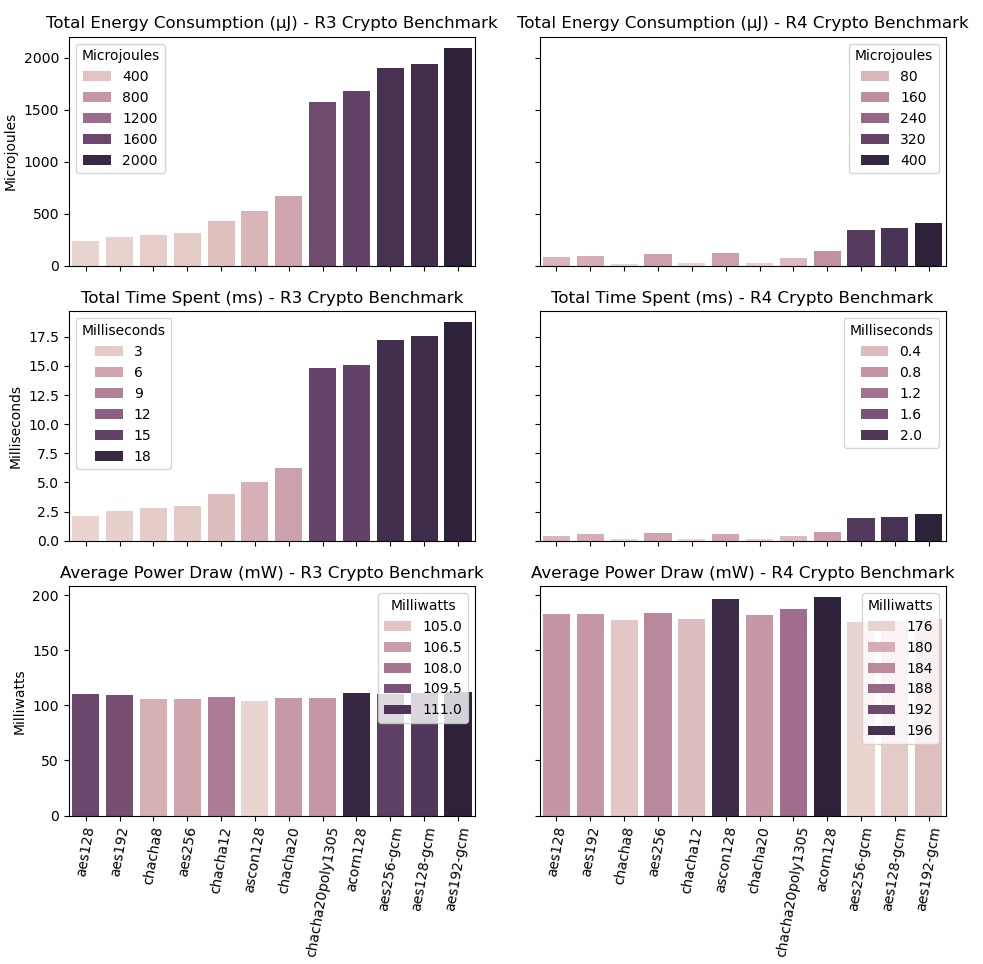
\includegraphics[scale=0.23]{crypto-results-r3-r4.png}
	\shorthandon{=} %\usepackage[turkish]{babel} kullanıldığı için komuta gerek var
	\caption{Kriptografi algoritmalarının R3 ve R4'teki performansları}
	\label{crypto-r3-r4}
\end{figure}
\pagebreak
\figurename~\ref{crypto-r3-r4}’deki kriptografik algoritmalarla ilgili olarak, sonuçlar cihaza bağlı olarak değişmektedir. R3'te Ascon128’nin AEAD algoritmalarında genel olarak en verimli olduğu tespit edilmiştir. Temel algoritmalar arasında AES'in en verimli olduğu tespit edilmiştir, ancak genel kullanım için AEAD'lar önerilmektedir \cite{cryptography-engineering}. R4'te ChaCha20Poly1305'in genel olarak en verimli olduğu, ChaCha yordamlarının ise AES ve Acorn128/Ascon128’den daha verimli olduğu görülmüştür. AES altyordamlarının tamamen yazılım tabanlı bir implementasyon olduğu ve donanım hızlandırma kullanılmadığı burada önemli bir husustur. \figurename~\ref{llmsort-r4}’teki LLM karşılaştırılmalarında ChatGPT'nin ortalama olarak Gemini'dan \%3,09 daha verimli, Claude'dan ise \%3,67 daha verimli kod ürettiği, ancak genellikle birbirlerine çok yakın sonuçlar verdiği görülmüştür.


\begin{figure}[h]
	\centering
	\shorthandoff{=}  %\usepackage[turkish]{babel} kullanıldığı için komuta gerek var
	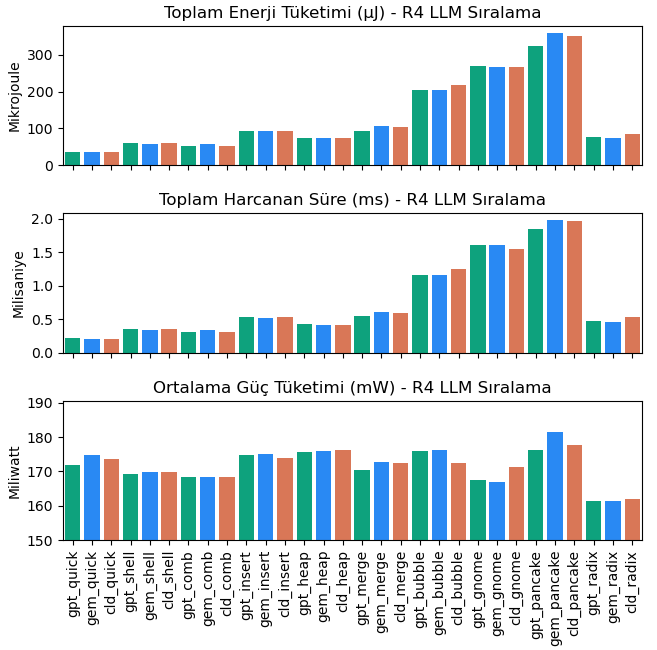
\includegraphics[scale=0.38]{llmsort-r4-renkli-v4.png}
	\shorthandon{=} %\usepackage[turkish]{babel} kullanıldığı için komuta gerek var
	\caption{Büyük dil modellerinin R4 için yazdığı algoritmaların performansları}
	\label{llmsort-r4}
\end{figure}

R3'ün performansta bir düşüş yaşamadan 2,735V'luk bir güç kaynağı ile çalışabildiği, bunun da enerji kullanımını azalttığı görülmüştür. Ancak stabilite için kartın daha yüksek bir gerilimle çalıştırılması tavsiye edilmektedir. Genel olarak, R4'ün hem daha hızlı hem de daha verimli olduğu tespit edilmiştir. Bu sonuç, R4'ün daha modern ve daha verimli mikroişlemci mimarisine sahip olmasına bağlanmıştır.

\section{Sonuç}

Bu araştırma, algoritmaların güç tüketimlerini zaman karmaşıklıklarıyla ilişkilendirerek incelemiştir. Yapılan deneyler, enerji tüketimi ile algoritmaların zaman karmaşıklığı arasında doğrudan bir ilişki olduğunu göstermektedir. Özellikle sıralama algoritmalarının enerji verimliliği analiz edildiğinde, Quick Sort gibi zaman verimli algoritmaların enerji tüketimi açısından da avantajlı olduğu gözlemlenmiştir. Bununla birlikte, farklı platformlar üzerinde yapılan testler, Radix Sort gibi belirli algoritmaların güç tüketiminin, kullanılan donanımın özellikleriyle de yakından ilişkili olduğunu ortaya koymuştur. Zaman karmaşıklığına dayalı optimizasyonların, enerji verimliliği sağlamak adına önemli bir rol oynadığı, bu araştırma ile kanıtlanmıştır. Ayrıca büyük dil modelleri arasında yapılan analizde enerji verimliliği açısından \%3'e kadar çıkan farklar gözlemlenmiştir.

Sonuç olarak, bu çalıisma gömülü sistemler için enerji optimizasyonunun, algoritma seçiminden donanım mimarisine kadar birçok faktöre bağlı olduğunu ortaya koymuştur. Bu alandaki bulgular, hem teoriye dayalı hem de uygulamalı enerji verimliliği analizlerinin gelecekteki gömülü yazılım geliştirme süreçlerinde daha etkin bir şekilde kullanılabileceğini işaret etmektedir. Büyük dil modelleri üzerine olan bulgular gelecekteki bir araştırmada daha detaylı incelenecektir. Araştırma kapsamında alınan ölçümler, çalıştırılan kodlar ve detaylı deney bilgisi herkese açık bir GitHub deposuna\cite{github} yüklenecektir.


% no \IEEEPARstart

% You must have at least 2 lines in the paragraph with the drop letter

% (should never be an issue)

% An example of a floating figure using the graphicx package.
% Note that \label must occur AFTER (or within) \caption.
% For figures, \caption should occur after the \includegraphics.
% Note that IEEEtran v1.7 and later has special internal code that
% is designed to preserve the operation of \label within \caption
% even when the captionsoff option is in effect. However, because
% of issues like this, it may be the safest practice to put all your
% \label just after \caption rather than within \caption{}.
%
% Reminder: the "draftcls" or "draftclsnofoot", not "draft", class
% option should be used if it is desired that the figures are to be
% displayed while in draft mode.
%
%\begin{figure}[!t]
%\centering
%\includegraphics[width=2.5in]{myfigure}
% where an .eps filename suffix will be assumed under latex,
% and a .pdf suffix will be assumed for pdflatex; or what has been declared
% via \DeclareGraphicsExtensions.
%\caption{Simulation Results}
%\label{fig_sim}
%\end{figure}

% Note that IEEE typically puts floats only at the top, even when this
% results in a large percentage of a column being occupied by floats.

% An example of a double column floating figure using two subfigures.
% (The subfig.sty package must be loaded for this to work.)
% The subfigure \label commands are set within each subfloat command, the
% \label for the overall figure must come after \caption.
% \hfil must be used as a separator to get equal spacing.
% The subfigure.sty package works much the same way, except \subfigure is
% used instead of \subfloat.
%
%\begin{figure*}[!t]
%\centerline{\subfloat[Case I]\includegraphics[width=2.5in]{subfigcase1}%
%\label{fig_first_case}}
%\hfil
%\subfloat[Case II]{\includegraphics[width=2.5in]{subfigcase2}%
%\label{fig_second_case}}}
%\caption{Simulation results}
%\label{fig_sim}
%\end{figure*}
%
% Note that often IEEE papers with subfigures do not employ subfigure
% captions (using the optional argument to \subfloat), but instead will
% reference/describe all of them (a), (b), etc., within the main caption.


% An example of a floating table. Note that, for IEEE style tables, the
% \caption command should come BEFORE the table. Table text will default to
% \footnotesize as IEEE normally uses this smaller font for tables.
% The \label must come after \caption as always.
%
%\begin{table}[!t]
%% increase table row spacing, adjust to taste
%\renewcommand{\arraystretch}{1.3}
% if using array.sty, it might be a good idea to tweak the value of
% \extrarowheight as needed to properly center the text within the cells
%\caption{An Example of a Table}
%\label{table_example}
%\centering
%% Some packages, such as MDW tools, offer better commands for making tables
%% than the plain LaTeX2e tabular which is used here.
%\begin{tabular}{|c||c|}
%\hline
%One & Two\\
%\hline
%Three & Four\\
%\hline
%\end{tabular}
%\end{table}


% Note that IEEE does not put floats in the very first column - or typically
% anywhere on the first page for that matter. Also, in-text middle ("here")
% positioning is not used. Most IEEE journals/conferences use top floats
% exclusively. Note that, LaTeX2e, unlike IEEE journals/conferences, places
% footnotes above bottom floats. This can be corrected via the \fnbelowfloat
% command of the stfloats package.


% use section* for acknowledgement
%\section*{TEŞEKKÜR}
%Yazarın teşekkür etmek istediği kurum yada kişiler burada belirtilecek.

% trigger a \newpage just before the given reference
% number - used to balance the columns on the last page
% adjust value as needed - may need to be readjusted if
% the document is modified later
%\IEEEtriggeratref{8}
% The "triggered" command can be changed if desired:
%\IEEEtriggercmd{\enlargethispage{-5in}}

\section*{B{\footnotesize İ}lg{\footnotesize İ}lend{\footnotesize İ}rme}

 \textit{Bilgilendirmeler Gizlenmiştir}

% references section

% can use a bibliography generated by BibTeX as a .bbl file
% BibTeX documentation can be easily obtained at:
% http://www.ctan.org/tex-archive/biblio/bibtex/contrib/doc/
% The IEEEtran BibTeX style support page is at:
% http://www.michaelshell.org/tex/ieeetran/bibtex/
%\bibliographystyle{IEEEtran}
% argument is your BibTeX string definitions and bibliography database(s)
%\bibliography{IEEEabrv,../bib/paper}
%
% <OR> manually copy in the resultant .bbl file
% set second argument of \begin to the number of references
% (used to reserve space for the reference number labels box)

\begin{thebibliography}{1}

\bibitem{github}
https://github.com/xxxxxxxx/xxxxxxxx (\textit{Link Gizlenmiştir.})

\bibitem{iot-market-2024-summer}
IoT Analytics GmbH, “Connected IoT device market update—Summer 2024,” 2024. https://web.archive.org/web/20250222024327/https://iot-analytics.com/number-connected-iot-devices/ (erişildi Mar. 09, 2025).

\bibitem{bces-embedded-performance-energy-consumption-eval}
B. C. E. S. Nogueira et al., “Performance and Energy Consumption Evaluation of Embedded Applications: A Method Based on Platform’s Behavioral Model,” 21st International Symposium on Computer Architecture and High Performance Computing, pp. 135–142, Oct. 2009, doi: 10.1109/sbac-pad.2009.27.

\bibitem{tiwari-power-analysis}
V. Tiwari, S. Malik, and A. Wolfe, “Power analysis of embedded software: a first step towards software power minimization,” IEEE Transactions on Very Large Scale Integration (VLSI) Systems, vol. 2, no. 4, pp. 437–445, Dec. 1994, doi: 10.1109/92.335012.

\bibitem{steinke-instruction-level-energy-model}
S. Steinke, M. Knauer, L. Wehmeyer, P. Marwedel, "An accurate and
fine grain instruction-level energy model supporting software optimizations," In Proceedings of the International Symposium on Power And Timing Modeling, Optimizations and Simulation (PATMOS), Eylül 2001.

\bibitem{bunse-no-corr}
C. Bunse, H. Höpfner, E. Mansour, ve S. Roychoudhury, “Exploring the Energy Consumption of Data Sorting Algorithms in Embedded and Mobile Environments”, 2009 Tenth International Conference on Mobile Data Management: Systems, Services and Middleware. IEEE, ss. 600-607, 2009. doi: 10.1109/mdm.2009.103. 

\bibitem{hashimi-binary}
M. Al-Hashimi ve N. Aljabri, “Exploring Power Advantage of Binary Search: An Experimental Study”, International Journal of Advanced Computer Science and Applications, c. 13, sy 10. The Science and Information Organization, 2022. doi: 10.14569/ijacsa.2022.0131094.

\bibitem{hashimi-mergesort}
N. Aljabri, M. Al-Hashimi, M. Saleh, ve O. Abulnaja, “Investigating power efficiency of mergesort”, The Journal of Supercomputing, c. 75, sy 10. Springer Science and Business Media LLC, ss. 6277-6302, Nis. 11, 2019. doi: 10.1007/s11227-019-02850-5. 

\bibitem{atmega328p-datasheet}
Microchip, “ATmega328P 8-bit AVR Microcontroller with 32K Bytes In-System Programmable Flash DATASHEET,” 2015. https://ww1.microchip.com/downloads/en/DeviceDoc/Atmel-7810-Automotive-Microcontrollers-ATmega328P\_Datasheet.pdf (erişildi Mar. 09, 2025).

\bibitem{ra4m1-datasheet}
Renesas Electronics, “RA4M1 Group Datasheet,” Sep. 29, 2023. https://www.renesas.com/en/document/dst/ra4m1-group-datasheet (erişildi Mar. 09, 2025).

\bibitem{nordic-ppk-datasheet}
Nordic Semiconductor ASA., “Power Profiler Kit II Technical Documentation,” 2025. https://docs.nordicsemi.com/bundle /ug\_ppk2/page/UG/ppk/PPK\_user\_guide\_Intro.html (erişildi Mar. 09, 2025).

\bibitem{cryptography-engineering}
N. Ferguson, B. Schneier, and T. Kohno, Cryptography Engineering: Design Principles and Practical Applications. Wiley, 2010, ss 220.

\end{thebibliography}


% that's all folks
\end{document} 